\documentclass{standalone}
\usepackage{tikz}
\usetikzlibrary{patterns, positioning}
\usepackage[sfdefault]{ClearSans} %% option 'sfdefault' activates Clear Sans as the default text font
\usepackage[T1]{fontenc}

\begin{document}
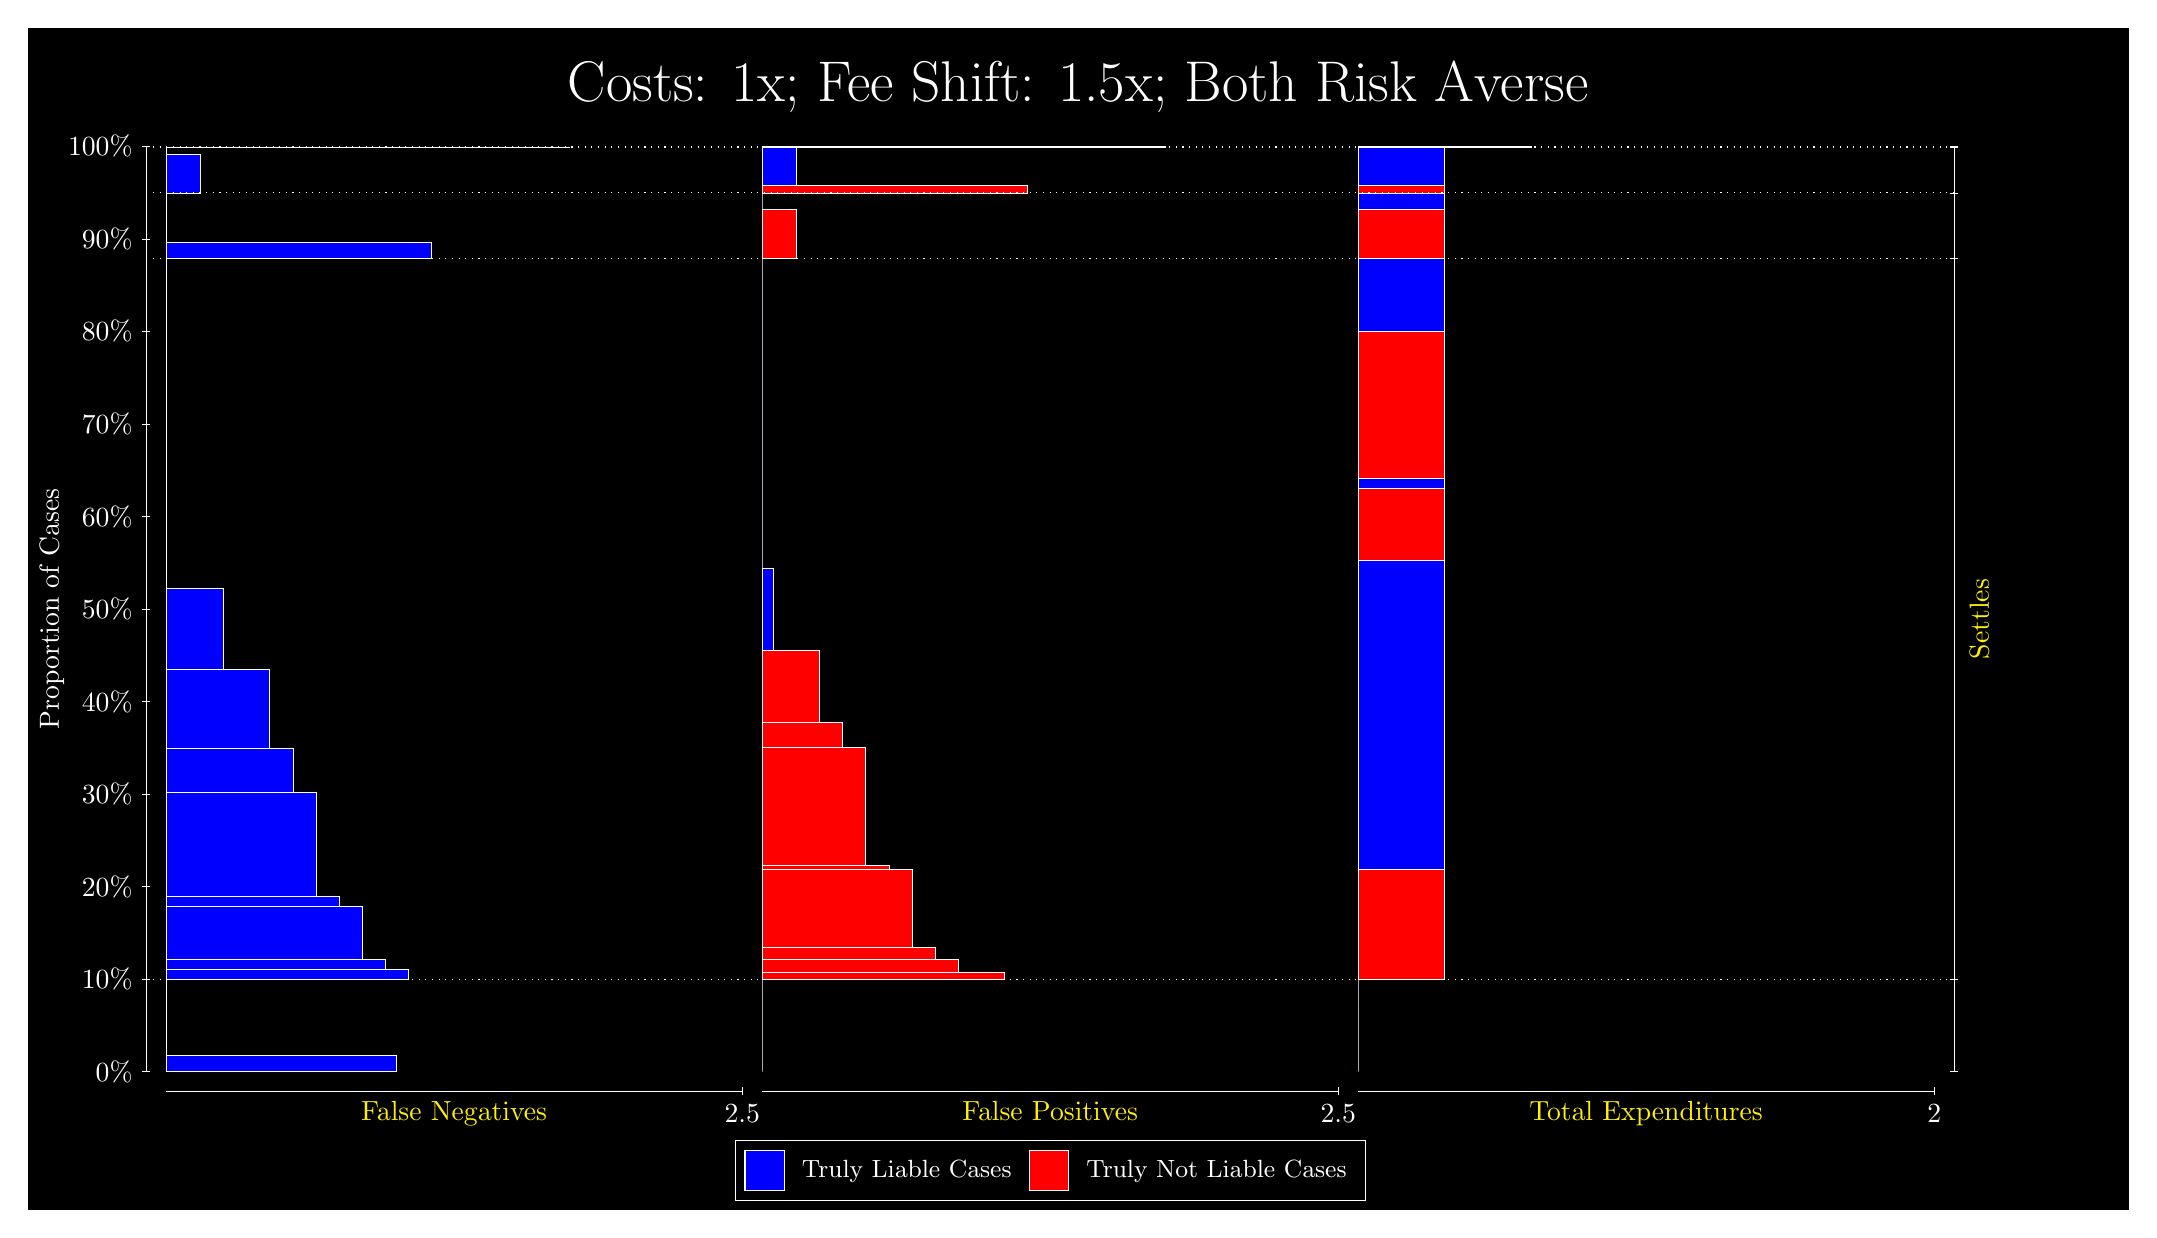
\begin{tikzpicture}
\draw[fill=black] (0,0) rectangle (26.667,15);
\draw[text=white] (0,13.5) rectangle (26.667,15) node[midway] {\huge Costs: 1x; Fee Shift: 1.5x; Both Risk Averse};
\draw[white, very thin] (1.5,1.75) -- (1.5,13.5);
\node[rotate=90, text=white, anchor=center] at (0.3, 7.625) {Proportion of Cases};
\draw[white, very thin] (1.45,1.75) -- (1.55,1.75);
\node[text=white, anchor=east] at (1.45, 1.75) {0\%};
\draw[white, very thin] (1.45,2.925) -- (1.55,2.925);
\node[text=white, anchor=east] at (1.45, 2.925) {10\%};
\draw[white, very thin] (1.45,4.1) -- (1.55,4.1);
\node[text=white, anchor=east] at (1.45, 4.1) {20\%};
\draw[white, very thin] (1.45,5.275) -- (1.55,5.275);
\node[text=white, anchor=east] at (1.45, 5.275) {30\%};
\draw[white, very thin] (1.45,6.45) -- (1.55,6.45);
\node[text=white, anchor=east] at (1.45, 6.45) {40\%};
\draw[white, very thin] (1.45,7.625) -- (1.55,7.625);
\node[text=white, anchor=east] at (1.45, 7.625) {50\%};
\draw[white, very thin] (1.45,8.8) -- (1.55,8.8);
\node[text=white, anchor=east] at (1.45, 8.8) {60\%};
\draw[white, very thin] (1.45,9.975) -- (1.55,9.975);
\node[text=white, anchor=east] at (1.45, 9.975) {70\%};
\draw[white, very thin] (1.45,11.15) -- (1.55,11.15);
\node[text=white, anchor=east] at (1.45, 11.15) {80\%};
\draw[white, very thin] (1.45,12.325) -- (1.55,12.325);
\node[text=white, anchor=east] at (1.45, 12.325) {90\%};
\draw[white, very thin] (1.45,13.5) -- (1.55,13.5);
\node[text=white, anchor=east] at (1.45, 13.5) {100\%};

\draw[white, very thin] (24.457,1.75) -- (24.457,13.5);
\draw[white, very thin] (24.407,1.75) -- (24.507,1.75);
\node[anchor=west] at (24.407, 1.75) {};
\draw[white, very thin] (24.407,2.9205) -- (24.507,2.9205);
\node[anchor=west] at (24.407, 2.9205) {};
\draw[white, very thin] (24.407,12.074) -- (24.507,12.074);
\node[anchor=west] at (24.407, 12.074) {};
\draw[white, very thin] (24.407,12.908) -- (24.507,12.908);
\node[anchor=west] at (24.407, 12.908) {};
\draw[white, very thin] (24.407,13.487) -- (24.507,13.487);
\node[anchor=west] at (24.407, 13.487) {};
\draw[white, very thin] (24.407,13.493) -- (24.507,13.493);
\node[anchor=west] at (24.407, 13.493) {};
\draw[white, very thin] (24.407,13.5) -- (24.507,13.5);
\node[anchor=west] at (24.407, 13.5) {};

\draw[white, very thin, fill=blue] (1.75,1.75) rectangle (4.6775,1.9515);
\draw[white, very thin, fill=red] (1.75,1.9515) rectangle (1.75,2.9205);
\draw[white, very thin, fill=blue] (1.75,2.9205) rectangle (4.8239,3.0475);
\draw[white, very thin, fill=blue] (1.75,3.0475) rectangle (4.5312,3.1738);
\draw[white, very thin, fill=blue] (1.75,3.1738) rectangle (4.2384,3.8445);
\draw[white, very thin, fill=blue] (1.75,3.8445) rectangle (3.9457,3.9754);
\draw[white, very thin, fill=blue] (1.75,3.9754) rectangle (3.6529,5.3023);
\draw[white, very thin, fill=blue] (1.75,5.3023) rectangle (3.3602,5.8607);
\draw[white, very thin, fill=blue] (1.75,5.8607) rectangle (3.0674,6.8555);
\draw[white, very thin, fill=blue] (1.75,6.8555) rectangle (2.4819,7.8915);
\draw[white, very thin, fill=red] (1.75,7.8915) rectangle (1.75,12.074);
\draw[white, very thin, fill=blue] (1.75,12.074) rectangle (5.1167,12.281);
\draw[white, very thin, fill=red] (1.75,12.281) rectangle (1.75,12.908);
\draw[white, very thin, fill=blue] (1.75,12.908) rectangle (2.1891,13.396);
\draw[white, very thin, fill=red] (1.75,13.396) rectangle (1.75,13.487);
\draw[white, very thin, fill=blue] (1.75,13.487) rectangle (6.8732,13.49);
\draw[white, very thin, fill=red] (1.75,13.49) rectangle (1.75,13.493);
\draw[white, very thin, fill=red] (1.75,13.493) rectangle (1.75,13.496);
\draw[white, very thin, fill=blue] (1.75,13.496) rectangle (1.75,13.5);
\draw[white, very thin, fill=red] (9.3189,1.75) rectangle (9.3189,2.719);
\draw[white, very thin, fill=blue] (9.3189,2.719) rectangle (9.3189,2.9205);
\draw[white, very thin, fill=red] (9.3189,2.9205) rectangle (12.393,3.005);
\draw[white, very thin, fill=red] (9.3189,3.005) rectangle (11.807,3.1753);
\draw[white, very thin, fill=red] (9.3189,3.1753) rectangle (11.515,3.3299);
\draw[white, very thin, fill=red] (9.3189,3.3299) rectangle (11.222,4.321);
\draw[white, very thin, fill=red] (9.3189,4.321) rectangle (10.929,4.3638);
\draw[white, very thin, fill=red] (9.3189,4.3638) rectangle (10.636,5.8667);
\draw[white, very thin, fill=red] (9.3189,5.8667) rectangle (10.344,6.1829);
\draw[white, very thin, fill=red] (9.3189,6.1829) rectangle (10.051,7.1025);
\draw[white, very thin, fill=blue] (9.3189,7.1025) rectangle (9.4652,8.1385);
\draw[white, very thin, fill=blue] (9.3189,8.1385) rectangle (9.3189,12.074);
\draw[white, very thin, fill=red] (9.3189,12.074) rectangle (9.758,12.701);
\draw[white, very thin, fill=blue] (9.3189,12.701) rectangle (9.3189,12.908);
\draw[white, very thin, fill=red] (9.3189,12.908) rectangle (12.686,12.999);
\draw[white, very thin, fill=blue] (9.3189,12.999) rectangle (9.758,13.487);
\draw[white, very thin, fill=red] (9.3189,13.487) rectangle (9.3189,13.491);
\draw[white, very thin, fill=blue] (9.3189,13.491) rectangle (9.3189,13.493);
\draw[white, very thin, fill=red] (9.3189,13.493) rectangle (14.442,13.496);
\draw[white, very thin, fill=blue] (9.3189,13.496) rectangle (11.515,13.5);
\draw[white, very thin, fill=red] (16.888,1.75) rectangle (16.888,2.719);
\draw[white, very thin, fill=blue] (16.888,2.719) rectangle (16.888,2.9205);
\draw[white, very thin, fill=red] (16.888,2.9205) rectangle (17.986,4.321);
\draw[white, very thin, fill=blue] (16.888,4.321) rectangle (17.986,8.2371);
\draw[white, very thin, fill=red] (16.888,8.2371) rectangle (17.986,9.1566);
\draw[white, very thin, fill=blue] (16.888,9.1566) rectangle (17.986,9.2837);
\draw[white, very thin, fill=red] (16.888,9.2837) rectangle (17.986,11.146);
\draw[white, very thin, fill=blue] (16.888,11.146) rectangle (17.986,12.074);
\draw[white, very thin, fill=red] (16.888,12.074) rectangle (17.986,12.701);
\draw[white, very thin, fill=blue] (16.888,12.701) rectangle (17.986,12.908);
\draw[white, very thin, fill=red] (16.888,12.908) rectangle (17.986,12.999);
\draw[white, very thin, fill=blue] (16.888,12.999) rectangle (17.986,13.487);
\draw[white, very thin, fill=red] (16.888,13.487) rectangle (19.083,13.491);
\draw[white, very thin, fill=blue] (16.888,13.491) rectangle (19.083,13.493);
\draw[white, very thin, fill=red] (16.888,13.493) rectangle (19.083,13.496);
\draw[white, very thin, fill=blue] (16.888,13.496) rectangle (19.083,13.5);
\draw[white, dotted] (1.5,2.9205) -- (24.457,2.9205);
\draw[white, dotted] (1.5,12.074) -- (24.457,12.074);
\draw[white, dotted] (1.5,12.908) -- (24.457,12.908);
\draw[white, dotted] (1.5,13.487) -- (24.457,13.487);
\draw[white, dotted] (1.5,13.493) -- (24.457,13.493);
\draw[white, very thin] (1.75,1.5) -- (9.0689,1.5);
\node[text=yellow, anchor=north] at (5.4094, 1.5) {False Negatives};
\draw[white, very thin] (9.0689,1.45) -- (9.0689,1.55);
\node[text=white, anchor=north] at (9.0689, 1.45) {2.5};

\draw[white, very thin] (9.3189,1.5) -- (16.638,1.5);
\node[text=yellow, anchor=north] at (12.978, 1.5) {False Positives};
\draw[white, very thin] (16.638,1.45) -- (16.638,1.55);
\node[text=white, anchor=north] at (16.638, 1.45) {2.5};

\draw[white, very thin] (16.888,1.5) -- (24.207,1.5);
\node[text=yellow, anchor=north] at (20.547, 1.5) {Total Expenditures};
\draw[white, very thin] (24.207,1.45) -- (24.207,1.55);
\node[text=white, anchor=north] at (24.207, 1.45) {2};


\node[text=yellow, centered, rotate=90] at (24.777, 7.497) {Settles};





\draw (12.978300999999998,1.5) node[draw=none] (baseCoordinate) {};
\begin{scope}[align=center]
        \matrix[scale=0.5, draw=white, below=0.5cm of baseCoordinate, nodes={draw}, column sep=0.1cm]{
            \node[rectangle, draw, minimum width=0.5cm, minimum height=0.5cm, fill=blue] {}; &
            \node[draw=none, font=\small, text=white] (B) {Truly Liable Cases}; &
            \node[rectangle, draw, minimum width=0.5cm, minimum height=0.5cm, fill=red] {}; &
            \node[draw=none, font=\small, text=white] (B) {Truly Not Liable Cases}; \\
            };
\end{scope}

\end{tikzpicture}
\end{document}